
\documentclass{article}
\usepackage[utf8]{inputenc}
\usepackage{geometry}
\geometry{a4paper, margin=1in}
\usepackage{graphicx}
\title{Utilizing Self-Rewarding Language Models for Anxiety Detection}
\author{Ian Li}
%\date{February 06, 2024}

\begin{document}

\maketitle

\section*{Proposal}


The advent of Self-Rewarding Language Models (SRLMs) heralds a transformative era in the field of Natural Language Processing (NLP), offering groundbreaking possibilities in various applications, including mental health. This project proposal delineates the application of SRLMs, as explicated in the seminal work "Self-Rewarding Language Models" (2024), to the domain of anxiety detection in textual data. SRLMs are distinguished by their unique self-improvement and evaluative capabilities, enabling them to generate, assess, and refine their own training data. This iterative process of self-evaluation and adaptation, also referred to as LLM-as-a-Judge prompting, allows the model to function both as a generator and a critic of its outputs, autonomously enhancing its performance based on self-assigned reward mechanisms.
\begin{center}
	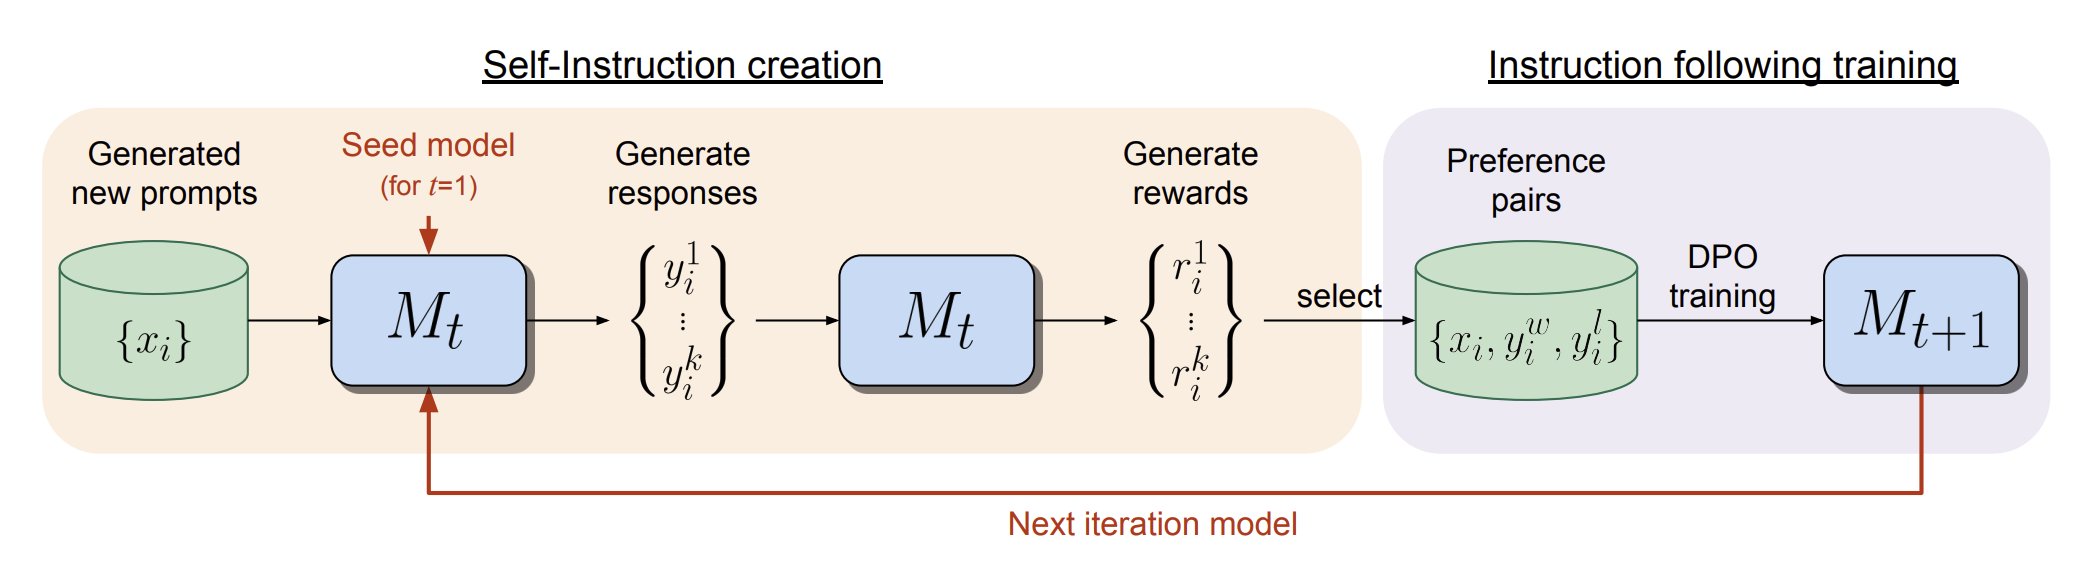
\includegraphics[scale=0.4]{srlm.png}
\end{center}


In the specific context of anxiety detection, the utilization of SRLMs involves the integration and analysis of extensive datasets encapsulating linguistic patterns and markers indicative of anxiety. This approach is predicated on the hypothesis that the self-rewarding mechanism intrinsic to these models will facilitate a nuanced and iterative refinement in their capability to identify and interpret subtle linguistic cues associated with anxiety. Consequently, this project aims to leverage the enhanced sensitivity and accuracy of SRLMs to detect and analyze expressions of anxiety in written text. Such an endeavor is anticipated to substantially augment the efficacy of current anxiety detection methodologies, thereby making a significant contribution to the domain of mental health diagnostics and intervention strategies.


This project proposal advocates for the application of Self-Rewarding Language Models (SRLMs) in the realm of anxiety detection in written text. SRLMs, a cutting-edge advancement in artificial intelligence, stand out due to their self-improving and evaluative capabilities, as outlined in recent literature (Self-Rewarding Language Models, 2023). These models are unique in their ability to generate and self-assess their own training data, continuously refining their performance. This self-evaluation process, termed LLM-as-a-Judge prompting, empowers the model to serve as its own judge, adjudicating rewards to its outputs based on predefined standards.

In the context of anxiety detection, leveraging SRLMs entails educating the model with varied datasets that incorporate linguistic markers indicative of anxiety. The innovative self-rewarding mechanism of these models facilitates an iterative refinement in understanding anxiety-related linguistic patterns. This enhancement in model sensitivity and accuracy is instrumental in detecting nuanced expressions of anxiety in text. The implementation of SRLMs in this domain promises to significantly improve the efficacy of anxiety detection tools, thereby contributing to more effective strategies in mental health diagnostics and intervention.

\end{document}
